\documentclass[conference]{IEEEtran}
\IEEEoverridecommandlockouts

\usepackage[utf8]{inputenc}
\usepackage{cite}
\usepackage{amsmath,amssymb,amsfonts}
\usepackage{graphicx}
\usepackage{subfig}
\usepackage{booktabs}
\usepackage{multirow}
\usepackage[ruled,vlined,linesnumbered]{algorithm2e}
\usepackage{tikz}
\usetikzlibrary{positioning,arrows.meta}
\usepackage[colorlinks=true,allcolors=blue]{hyperref}
\usepackage{float}
\usepackage{booktabs}

\SetKwInput{KwInput}{Input}
\SetKwInput{KwOutput}{Output}

\begin{document}

\title{ADARE: Adaptive Multi-Objective Scheduling for Edge/Fog/Cloud}

\author{
\IEEEauthorblockN{1\textsuperscript{st} Roland C\'edric TAYO}
\IEEEauthorblockA{\textit{CY Cergy Paris University, France}\\
rolandcedric.tayo@yahoo.fr}
\and
\IEEEauthorblockN{2\textsuperscript{nd} Sonia YASSA}
\IEEEauthorblockA{\textit{CY Cergy Paris University, France}\\
sonia.yassa@cyu.fr}
}

\maketitle

\begin{abstract}
Yesterday we were in the era of man interacting with the machine. Today, the machine interacts with other machines. The purpose of these exchanges is to produce and provide data even faster than yesterday. In order to achieve this feat, the machines distribute the tasks among themselves. Several algorithms make this possible, such as NSGA-III, which turns out to be one of the most effective. But we notice that most of these algorithms remain static in their approach.

This paper presents ADARE (Adaptive Deep-reinforced Auto-learning Resource Allocator Engine), a dynamic approach of adjusting its own parameters during a processing, in order to propose better distributions.

ADARE and NSGA-III taken on the basis of identical parameters (within 6 runs) have shown that ADARE wins the competition by proposing scores going up to $18/18$ in terms of quality and $15/15$ in terms of core-quality, for the datasets "Montage\_25", "CyberShake\_30" and "Epigenomics\_24". That is gains going up to $+36.18\%$ (core quality), $+9.45\%$ (best-objective metrics), and $+9.17\%$ (runtime)

We will explore throughout this document the 3 major algorithmic contributions of ADARE as well as the results of the tests conducted for our study.
\end{abstract}

\begin{IEEEkeywords}
Edge computing, Fog computing, Cloud computing, Multi-objective optimization, NSGA-III, Adaptive evolutionary algorithm
\end{IEEEkeywords}

\section{Introduction}
\subsection{Background and Motivation}
The Internet of Things (IoT) has invaded and conquered the routine of man. Behind these objects are hidden computing units represented by Edge, Fog and Cloud infrastructures. The selection of the ideal infrastructure to perform a computation influences the computation time, the response time, the energy consumption and by ricochet the financial costs.

These perpetually conflicting objectives are the constant optimization challenge that multi-objective optimization algorithms must overcome \cite{deb2014,deb2014nsga3}.

\subsection{Goals}
The fundamental goal is to find a common ground between these objectives, to optimize them. ADARE explores a dynamic and adaptive approach, while remaining fair-play during the evaluation. The goals are:
\begin{itemize}
    \item adapt operator behavior during search,
    \item keep Pareto diversity while improving convergence,
    \item improve objective extremes (especially makespan and latency),
    \item avoid runtime degradation.
\end{itemize}

\subsection{Paper Structure}
We have structured the paper as follows: Section II summarizes related approaches. Section III defines the optimization model. Section IV presents ADARE and its main algorithms. Section V gives the experimental setup. Section VI reports results. Section VII concludes.

\section{Related Work}
\subsection{Heuristic and Deterministic Schedulers}
Classical schedulers such as certain list-based heuristics are often very efficient when it comes to producing fast results. In heterogeneous edge/fog/cloud environments, this kind of algorithm would imply poor energy-cost trade-offs. Deterministic rules seriously lack efficiency when facing the highly variable characteristics of workloads.

\subsection{Evolutionary Many-Objective Methods}
Evolutionary methods balance conflicting objectives by maintaining non-dominated populations. NSGA-II and NSGA-III are standard baselines. NSGA-III turns out to be particularly suited to many-objective situations via reference-point selection \cite{deb2014nsga3}. But, when it comes to workflow scheduling, static crossover/mutation parameters can drastically reduce efficiency. Key operators could degrade the quality of solutions in later generations.

\subsection{Learning-Guided Hybrids}
Recent hybrid methods try to combine search and learning signals. But this approach often implies external pre-training or overly complicated and costly hyperparameter tuning. ADARE keeps the main learning loop light and online. Instead of replacing the evolutionary core, it injects adaptive mechanisms inside the loop itself : a crossover that adapts to the situation, a density-sensitive mutation (nothing is done randomly), and an archive-driven steering with final candidates converging toward the objectives. We learn better without building a factory of gas.

\section{Problem Modeling}
\subsection{System and Decision Model}
We schedule a workflow DAG $G=(V,E)$ over heterogeneous resources $R$ (edge/fog/cloud). Each task $v_i \in V$ has computational load and data transfer requirements. Each resource $r_k \in R$ has different processing rate, communication bandwidth, cost, and power profile.

An individual $x$ is a task-to-node assignment:
\begin{equation}
x = (x_1,\dots,x_{|V|}), \quad x_i \in \{1,\dots,|R|\}.
\end{equation}

\subsection{Objective Functions}
The objective vector is:
\begin{equation}
\min \mathbf{f}(x)=\big(f_{\text{makespan}},f_{\text{latency}},f_{\text{cost}},f_{\text{energy}}\big).
\end{equation}

Main components are:
\begin{itemize}
    \item $f_{\text{makespan}}=\max_i FT(v_i)$,
    \item $f_{\text{latency}}=\sum_i \big(FT(v_i)-RT(v_i)\big)$,
    \item $f_{\text{cost}}=\sum_i ET(v_i,x_i)\cdot C(x_i)$,
    \item $f_{\text{energy}}=\sum_i ET(v_i,x_i)\cdot P(x_i)$.
\end{itemize}

Here $FT$ is finish time, $RT$ is ready time under precedence constraints, and $ET$ is execution time on the assigned node.

\subsection{Optimization Target}
Our objectives are to :
\begin{itemize}
    \item a high-quality non-dominated front (HV, IGD, spacing, epsilon, coverage),
    \item robust objective extremes (best makespan, latency, cost, energy),
    \item competitive runtime.
\end{itemize}

\section{ADARE Methodology}
\subsection{Simple Structure Design}
\begin{figure}[H]
\centering
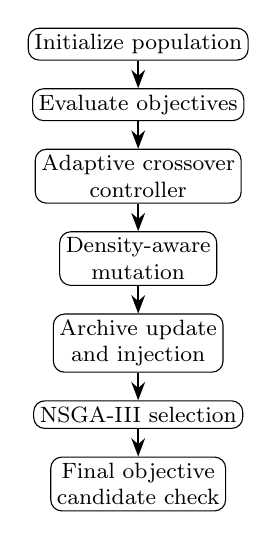
\begin{tikzpicture}[
node distance=3.5mm,
box/.style={draw, rounded corners, align=center, font=\footnotesize, inner sep=2.2pt},
arr/.style={-Stealth, thick}
]
\node[box] (init) {Initialize population};
\node[box, below=of init] (eval) {Evaluate objectives};
\node[box, below=of eval] (cross) {Adaptive crossover\\controller};
\node[box, below=of cross] (mut) {Density-aware\\mutation};
\node[box, below=of mut] (arch) {Archive update\\and injection};
\node[box, below=of arch] (sel) {NSGA-III selection};
\node[box, below=of sel] (final) {Final objective\\candidate check};
\draw[arr] (init) -- (eval);
\draw[arr] (eval) -- (cross);
\draw[arr] (cross) -- (mut);
\draw[arr] (mut) -- (arch);
\draw[arr] (arch) -- (sel);
\draw[arr] (sel) -- (final);
\end{tikzpicture}
\caption{Simple ADARE structure.}
\label{fig:adare_structure}
\end{figure}

\subsection{Contribution 1: Adaptive Crossover Control}
\begin{algorithm}[t]
\small
\caption{Adaptive Crossover Selection (RL-guided)}
\KwInput{Parents $p_1,p_2$, operator values $Q$, usage counts $N$, generation $g$}
\KwOutput{Children $c_1,c_2$, updated $Q,N$}
$\epsilon \leftarrow$ linear\_schedule$(g)$\;
\eIf{rand() $< \epsilon$}{
    $k \leftarrow$ random operator\;
}{
    $k \leftarrow \arg\max_i \left(Q_i + \sqrt{\frac{2\ln(\sum_j N_j+1)}{N_i+1}}\right)$\;
}
Apply crossover operator $k$ on $(p_1,p_2)$ to get $(c_1,c_2)$\;
$r \leftarrow \phi(\text{best}(p_1,p_2))-\phi(\text{best}(c_1,c_2))$\;
$Q_k \leftarrow (1-\alpha)Q_k + \alpha r$\;
$N_k \leftarrow N_k+1$\;
\end{algorithm}
This controller will progressively elect the best rewarded operators along the previous generations. The UCB term prevents the system from locking too early on a single operator.

\subsection{Contribution 2: Density-Aware Mutation}
\begin{algorithm}[t]
\small
\caption{Density-Aware Adaptive Mutation}
\KwInput{Individual $x$, diversity $d$, generation $g$, task-node rankings}
\KwOutput{Mutated individual $x'$}
$B \leftarrow$ dynamic mutation budget based on $(g,d)$\;
\For{$b=1$ \KwTo $B$}{
    pick task index $t$\;
    \eIf{rand() $< p_{heur}$}{
        assign $x_t$ from top-ranked nodes for task $t$\;
    }{
        assign $x_t$ to a random node\;
    }
}
apply low-probability gene-level mutation pass\;
$x' \leftarrow x$\;
\end{algorithm}
The more diversity decreases, the more mutation is stimulated in order to avoid any premature convergence. The structures obtained from previous generations are thus preserved.

\subsection{Contribution 3: Archive and Final Objective Candidates}
\begin{algorithm}[t]
\small
\caption{Archive-Guided Final Objective Pool}
\KwInput{Final population $P$, archive $A$, candidate keys $K$}
\KwOutput{$P$ (quality front), $P^{obj}$ (objective-extreme pool)}
$P^{obj} \leftarrow P \cup A$\;
\ForEach{$k \in K$}{
    evaluate candidate $k$\;
    \If{$k$ improves best makespan or best latency or best energy}{
        add $k$ to $P^{obj}$\;
    }
}
return $P$ for Pareto-quality metrics and $P^{obj}$ for objective-best metrics\;
\end{algorithm}
The most important point is to separate roles: Pareto quality is measured on the stable final front $P$, while objective extremes are validated on $P^{obj}$. This keeps front quality intact while allowing targeted objective improvements.

\section{Experimental Setup}
The comparison protocol is strictly the same for ADARE and NSGA-III to avoid any bias.
\begin{table}[htbp]
\centering
\caption{Shared Configuration}
\label{tab:shared}
\begin{tabular}{lcc}
\toprule
\textbf{Parameter} & \textbf{ADARE} & \textbf{NSGA-III} \\
\midrule
Population size & 100 & 100 \\
Generations & 70 & 70 \\
Crossover probability & 0.85 & 0.85 \\
Mutation probability & 0.20 & 0.20 \\
Gene mutation probability & 0.08 & 0.08 \\
Runs per benchmark & 6 & 6 \\
\bottomrule
\end{tabular}
\end{table}

\noindent Benchmarks: Montage\_25, CyberShake\_30, Epigenomics\_24.

\noindent Metrics: HV, IGD, spacing, epsilon, coverage, runtime, and best objective values.

\subsection{Fairness Controls}
For each run, we make sure that both algorithms start with the same initial population. For that, the same seed is used at the start.
The evaluator, the order of objectives, the hardware context and the generation budget are all identical.
We thus protect ourselves from any hidden advantage, linked to initialization or to differences in the way metrics are implemented.

\subsection{Statistical Protocol}
We retrieve, for each benchmark, means and standard deviations over 6 runs.
We also perform paired Wilcoxon tests to observe whether gain values are statistically significant across shared-seed runs.

\section{Results and Discussion}
\begin{table}[htbp]
\centering
\caption{Global Results (Latest 6-Run Campaign)}
\label{tab:global_results}
\begin{tabular}{lccc}
\toprule
\textbf{Benchmark} & \textbf{Core Gain} & \textbf{Obj. Gain} & \textbf{Time Gain} \\
\midrule
Montage\_25 & +36.31\% & +14.78\% & +6.93\% \\
CyberShake\_30 & +20.48\% & +10.59\% & +12.38\% \\
Epigenomics\_24 & +51.75\% & +2.98\% & +8.18\% \\
\midrule
\textbf{Mean} & \textbf{+36.18\%} & \textbf{+9.45\%} & \textbf{+9.17\%} \\
\bottomrule
\end{tabular}
\end{table}

\begin{table*}[htbp]
\centering
\caption{Detailed Metrics Snapshot (mean$\pm$std over 6 runs)}
\label{tab:detailed_snapshot}
\begin{tabular}{llccc}
\toprule
\textbf{Benchmark} & \textbf{Metric} & \textbf{ADARE} & \textbf{NSGA-III} & \textbf{Gain (\%)} \\
\midrule
Montage\_25 & HV & $0.91163\pm0.0108$ & $0.864108\pm0.0224$ & +5.50 \\
Montage\_25 & IGD & $0.0621207\pm0.00555$ & $0.0644155\pm0.00447$ & +3.56 \\
Montage\_25 & Time & $1.15959\pm0.034$ & $1.246\pm0.069$ & +6.93 \\
Montage\_25 & Makespan\_best & $2282.78\pm0$ & $2876.98\pm147$ & +20.65 \\
Montage\_25 & Latency\_best & $11160\pm0$ & $12744.5\pm535$ & +12.43 \\
\midrule
CyberShake\_30 & HV & $0.929627\pm0.00732$ & $0.89443\pm0.0104$ & +3.94 \\
CyberShake\_30 & IGD & $0.0698127\pm0.00494$ & $0.0745182\pm0.00348$ & +6.31 \\
CyberShake\_30 & Time & $1.29986\pm0.0803$ & $1.48357\pm0.123$ & +12.38 \\
CyberShake\_30 & Makespan\_best & $10806.6\pm0$ & $11416.4\pm515$ & +5.34 \\
CyberShake\_30 & Latency\_best & $47940\pm0$ & $52626.2\pm1.72\times10^3$ & +8.90 \\
\midrule
Epigenomics\_24 & HV & $1.1125\pm0.00156$ & $1.1046\pm0.00345$ & +0.72 \\
Epigenomics\_24 & IGD & $0.0381703\pm0.00329$ & $0.0401564\pm0.00321$ & +4.95 \\
Epigenomics\_24 & Time & $1.18571\pm0.0242$ & $1.29134\pm0.069$ & +8.18 \\
Epigenomics\_24 & Makespan\_best & $261644\pm0$ & $265167\pm7.4\times10^3$ & +1.33 \\
Epigenomics\_24 & Latency\_best & $830721\pm0$ & $874313\pm3.5\times10^4$ & +4.99 \\
\bottomrule
\end{tabular}
\end{table*}

Global outcomes: ADARE wins 18/18 quality slots and 15/15 core-quality slots. It also improves previously weak extremes:
\begin{itemize}
    \item CyberShake\_30: makespan\_best +5.34\%, latency\_best +8.90\%.
    \item Epigenomics\_24: makespan\_best +1.33\%, latency\_best +4.99\%.
\end{itemize}

\begin{table}[htbp]
\centering
\caption{Quality Metric Gains (\%) of ADARE over NSGA-III}
\label{tab:quality_gains}
\begin{tabular}{lccc}
\toprule
\textbf{Metric} & \textbf{Montage} & \textbf{CyberShake} & \textbf{Epigenomics} \\
\midrule
HV & +5.50 & +3.94 & +0.72 \\
IGD & +3.56 & +6.31 & +4.95 \\
Spacing & +16.73 & +1.89 & +27.83 \\
Epsilon & +21.35 & +17.84 & +5.64 \\
Coverage & +134.40 & +72.42 & +219.59 \\
Runtime & +6.93 & +12.38 & +8.18 \\
\bottomrule
\end{tabular}
\end{table}

\begin{table}[htbp]
\centering
\caption{Best-Objective Gains (\%) of ADARE}
\label{tab:objective_gains}
\begin{tabular}{lccc}
\toprule
\textbf{Metric} & \textbf{Montage} & \textbf{CyberShake} & \textbf{Epigenomics} \\
\midrule
Makespan\_best & +20.65 & +5.34 & +1.33 \\
Latency\_best & +12.43 & +8.90 & +4.99 \\
Cost\_best & +23.27 & +26.08 & +5.48 \\
Energy\_best & +2.76 & +2.03 & +0.14 \\
\bottomrule
\end{tabular}
\end{table}

\begin{figure*}[t]
\centering
\subfloat[Montage\_25]{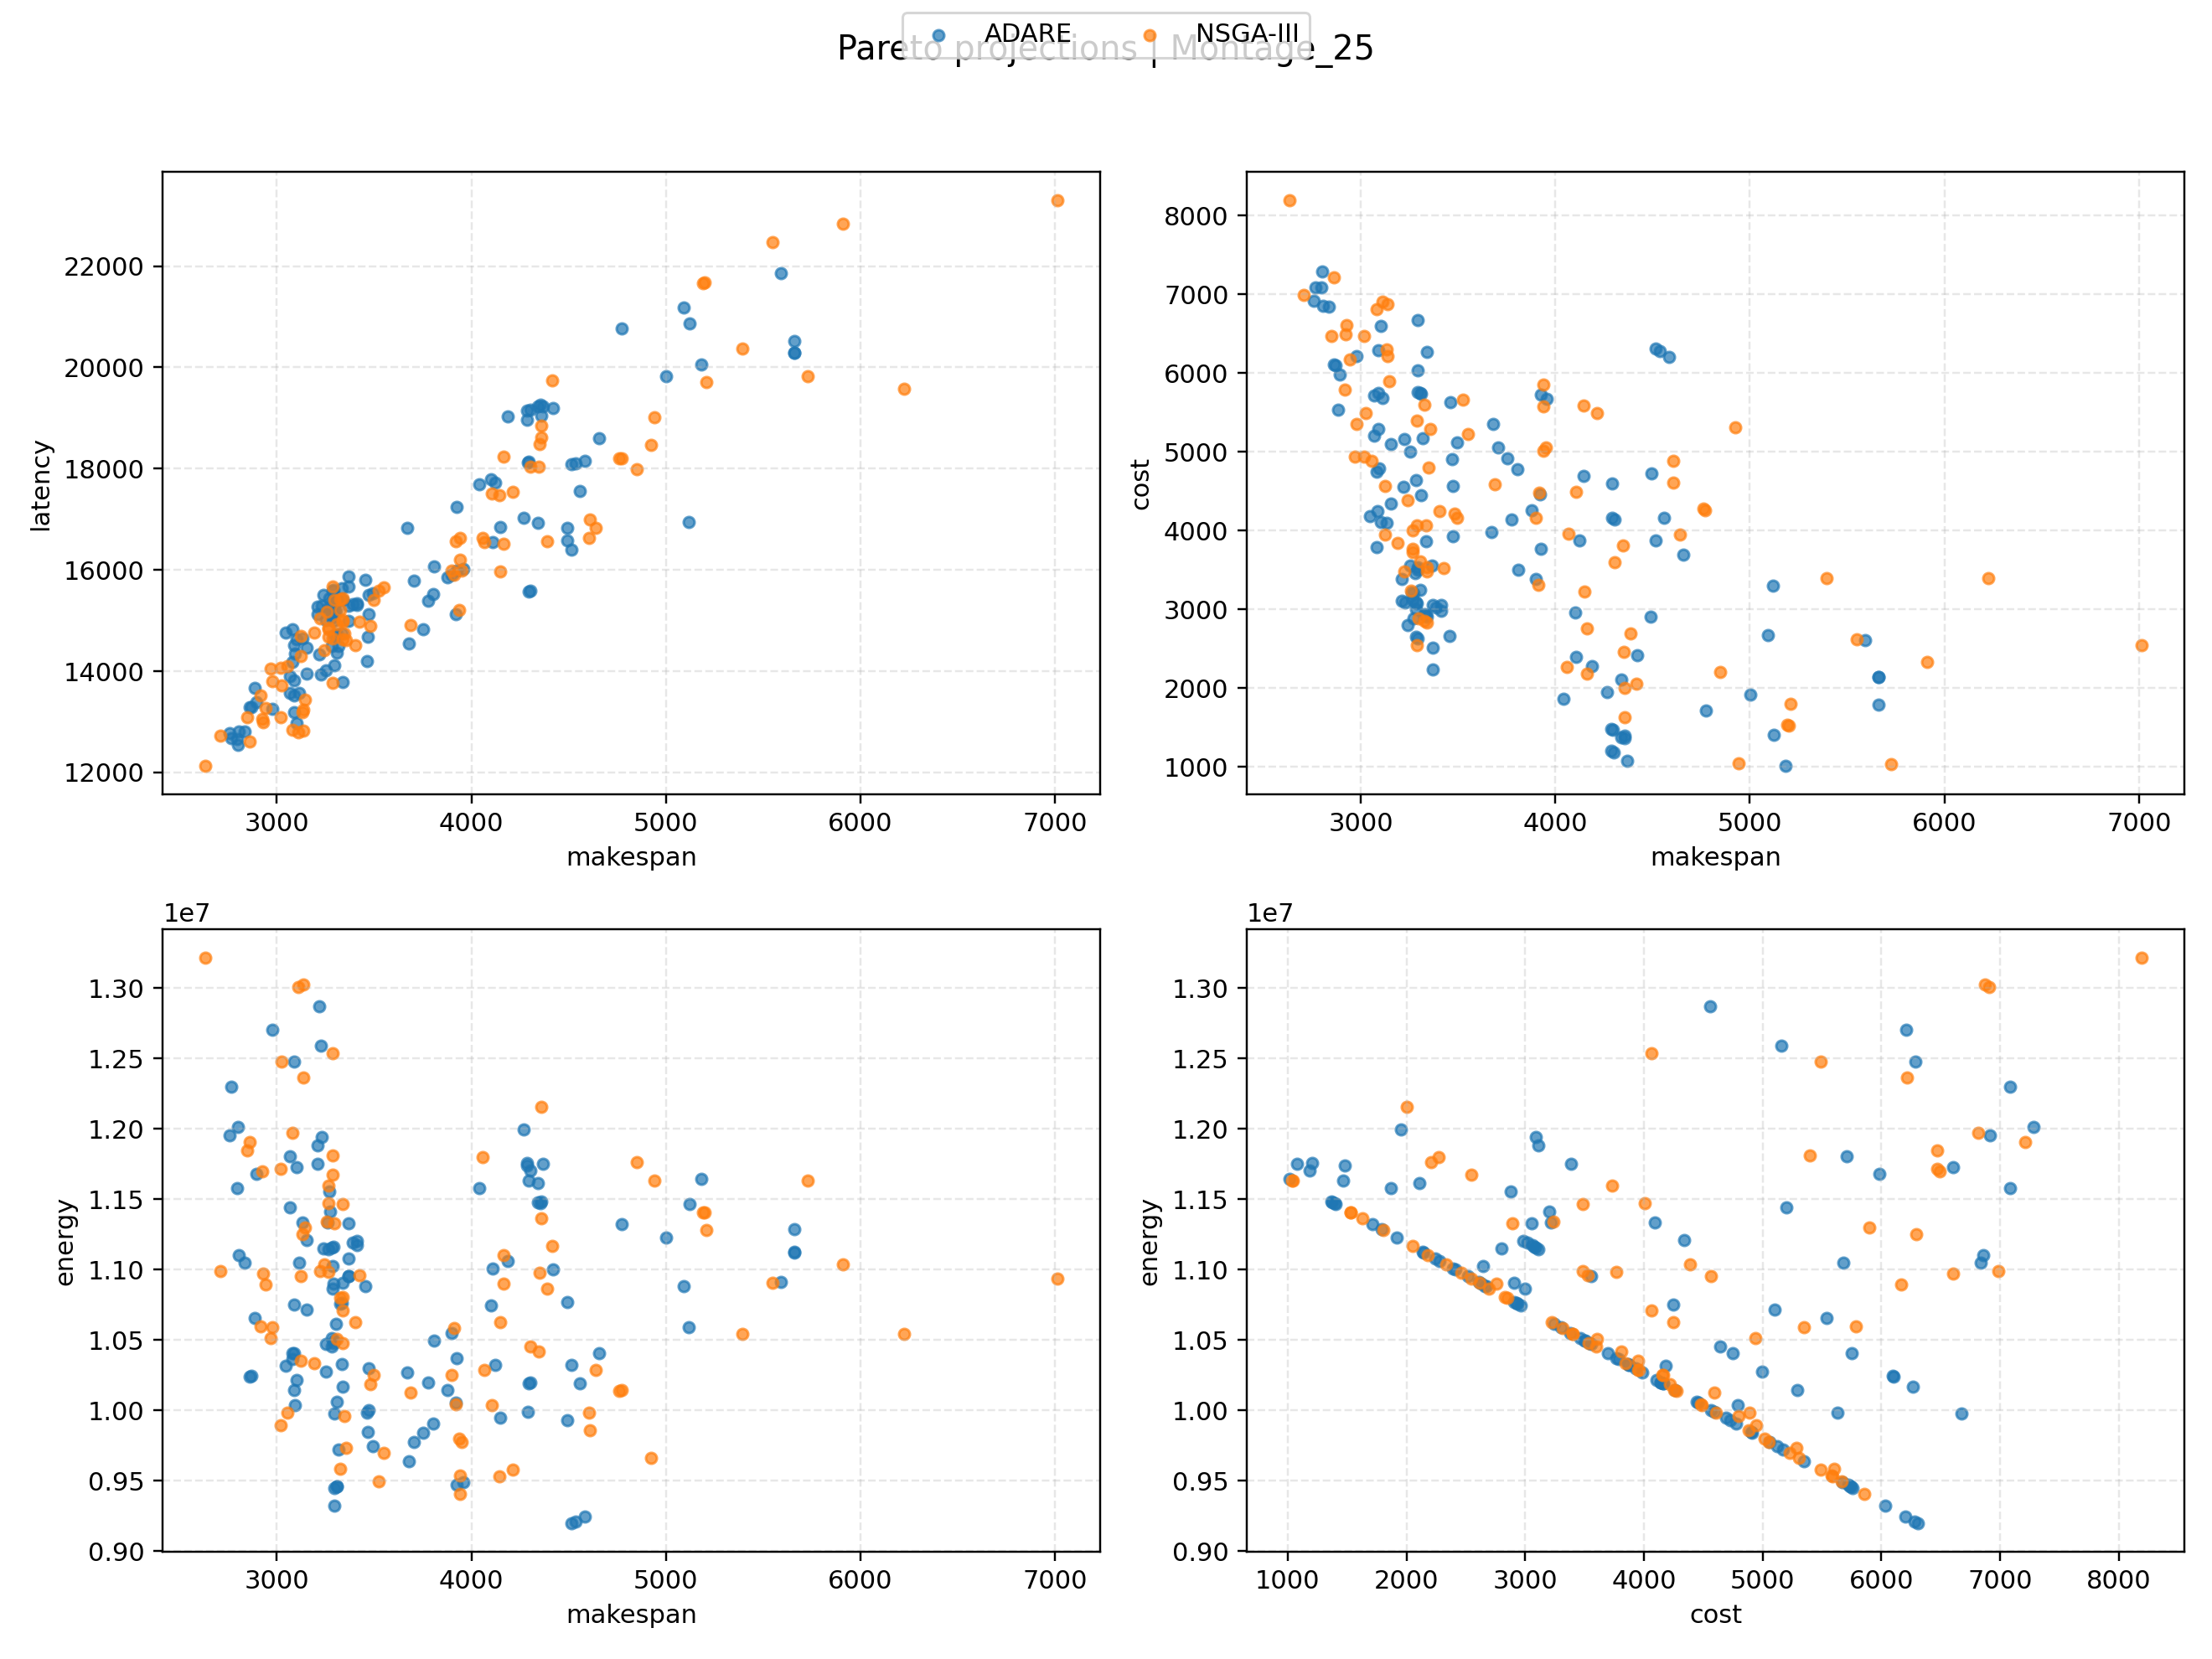
\includegraphics[width=0.32\textwidth]{Figures/pareto_test_montage25.png}}
\hfill
\subfloat[CyberShake\_30]{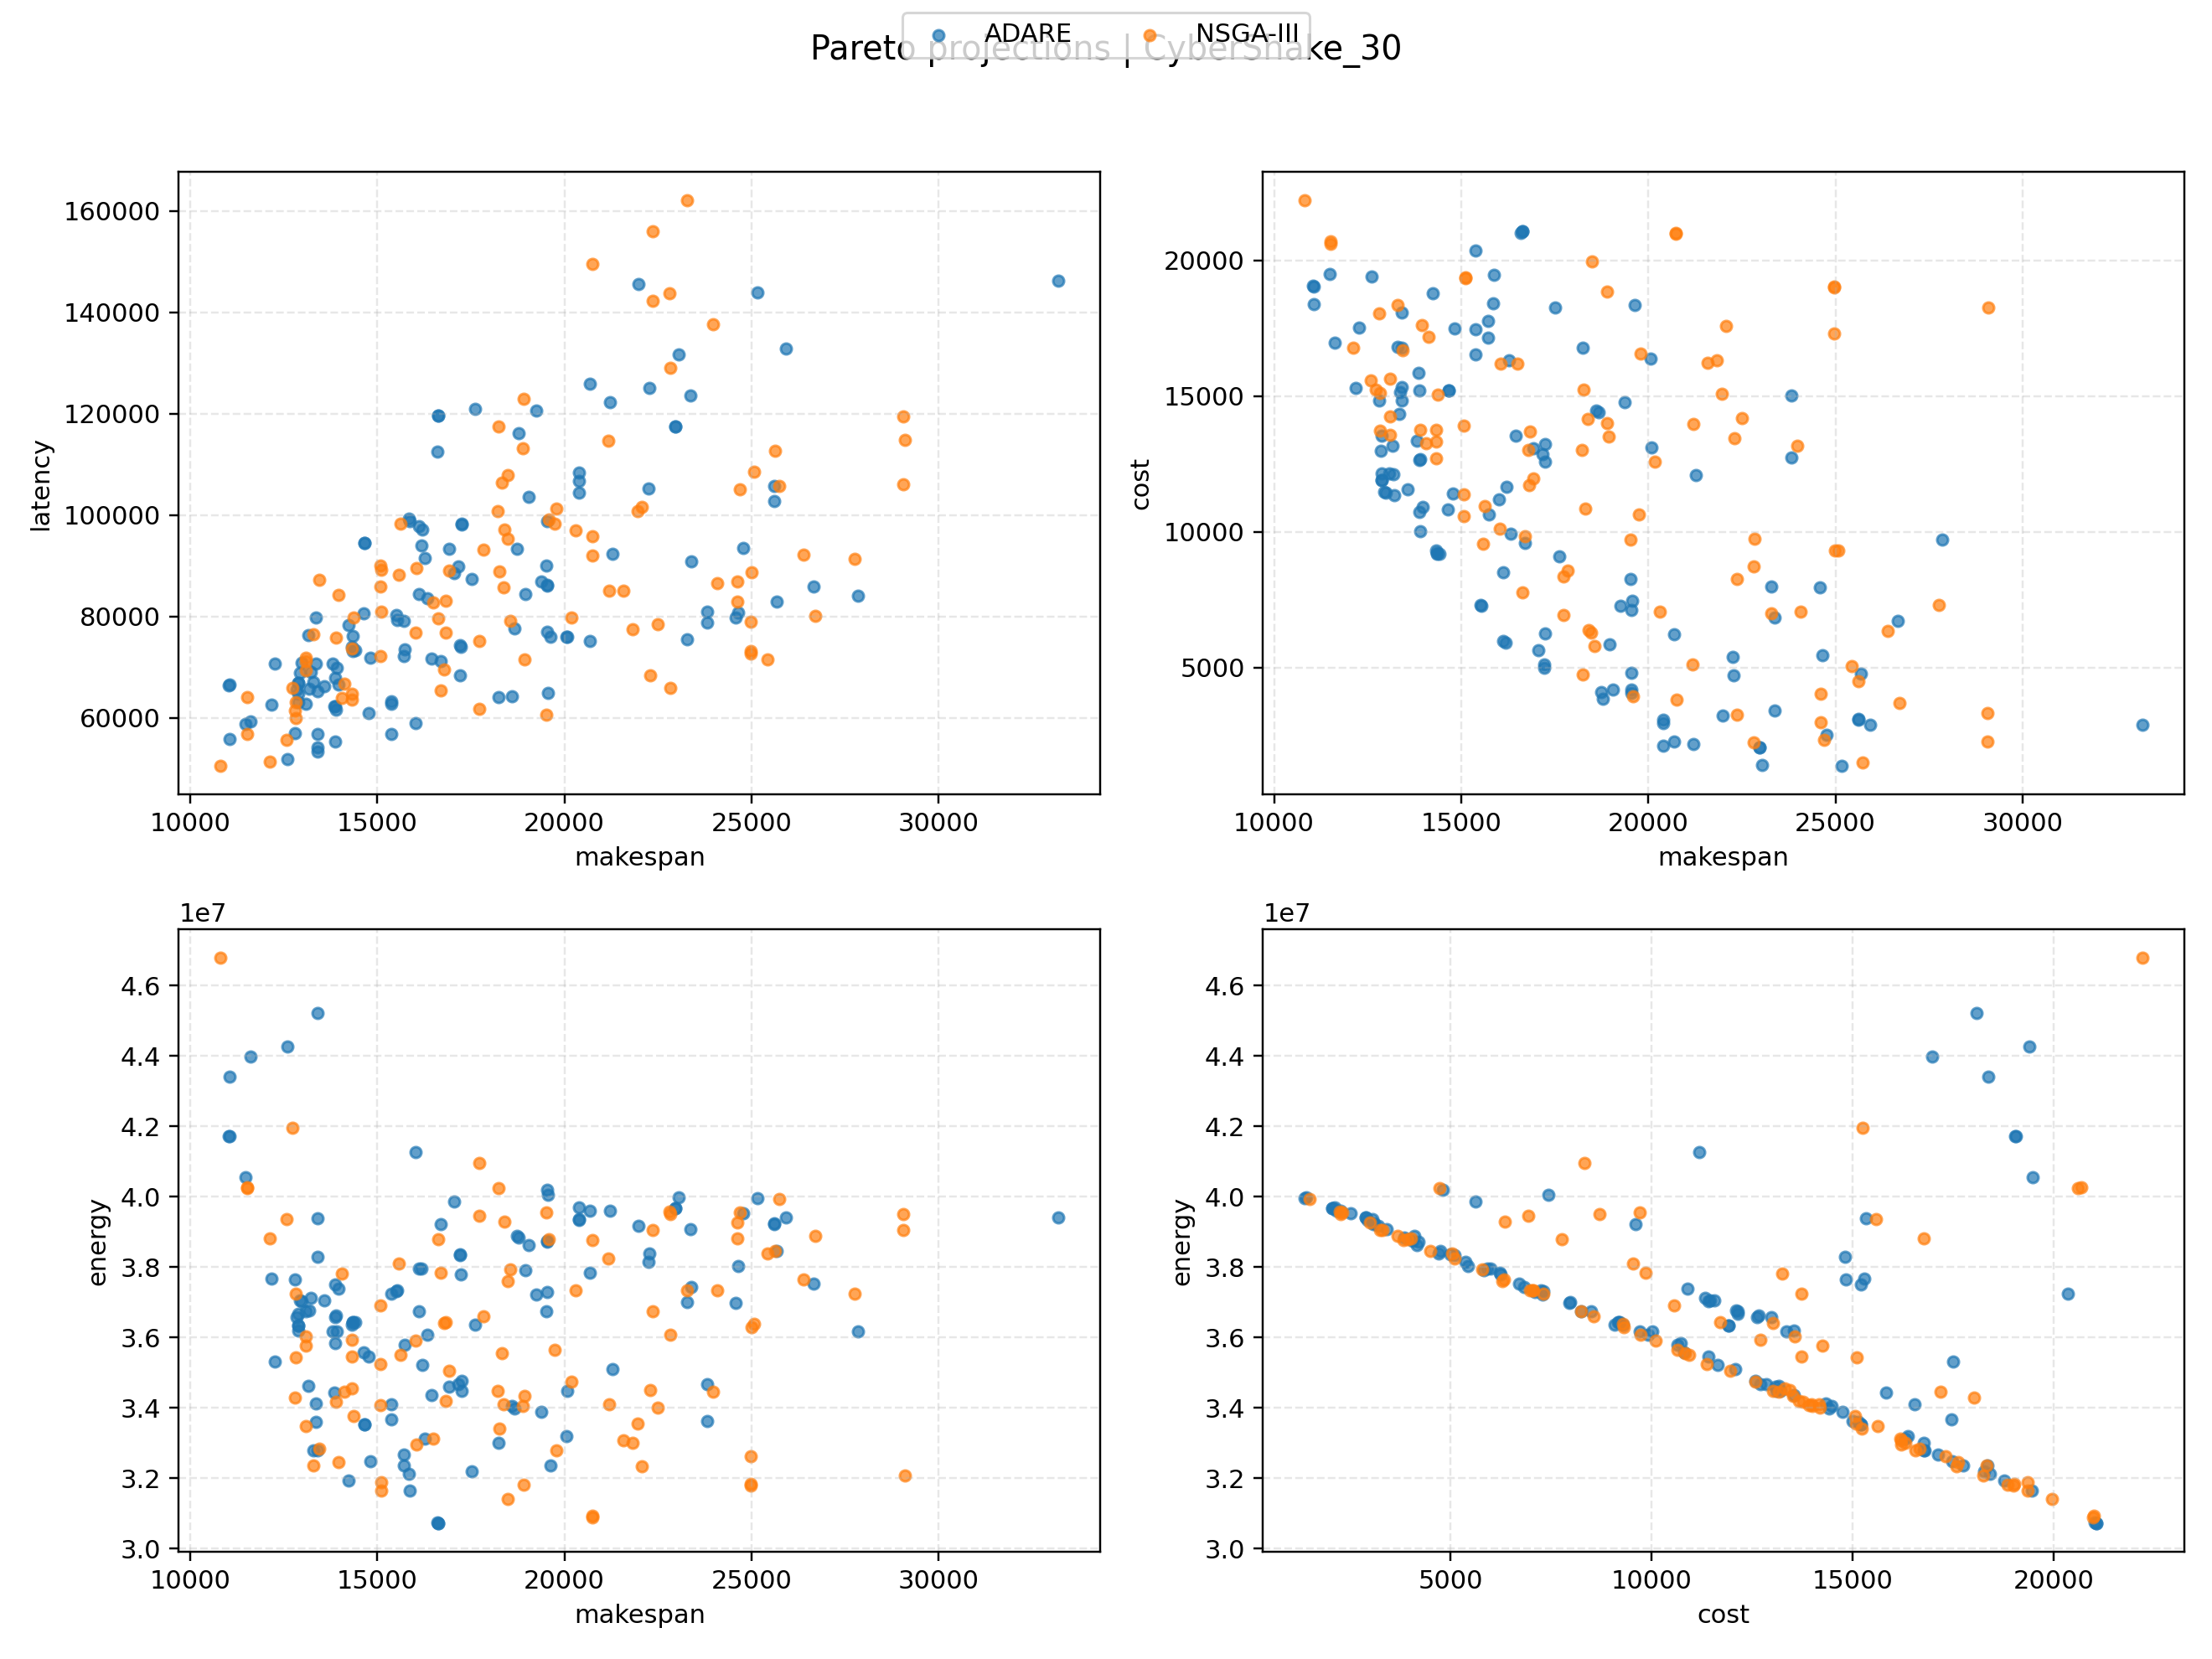
\includegraphics[width=0.32\textwidth]{Figures/pareto_test_cybershake30.png}}
\hfill
\subfloat[Epigenomics\_24]{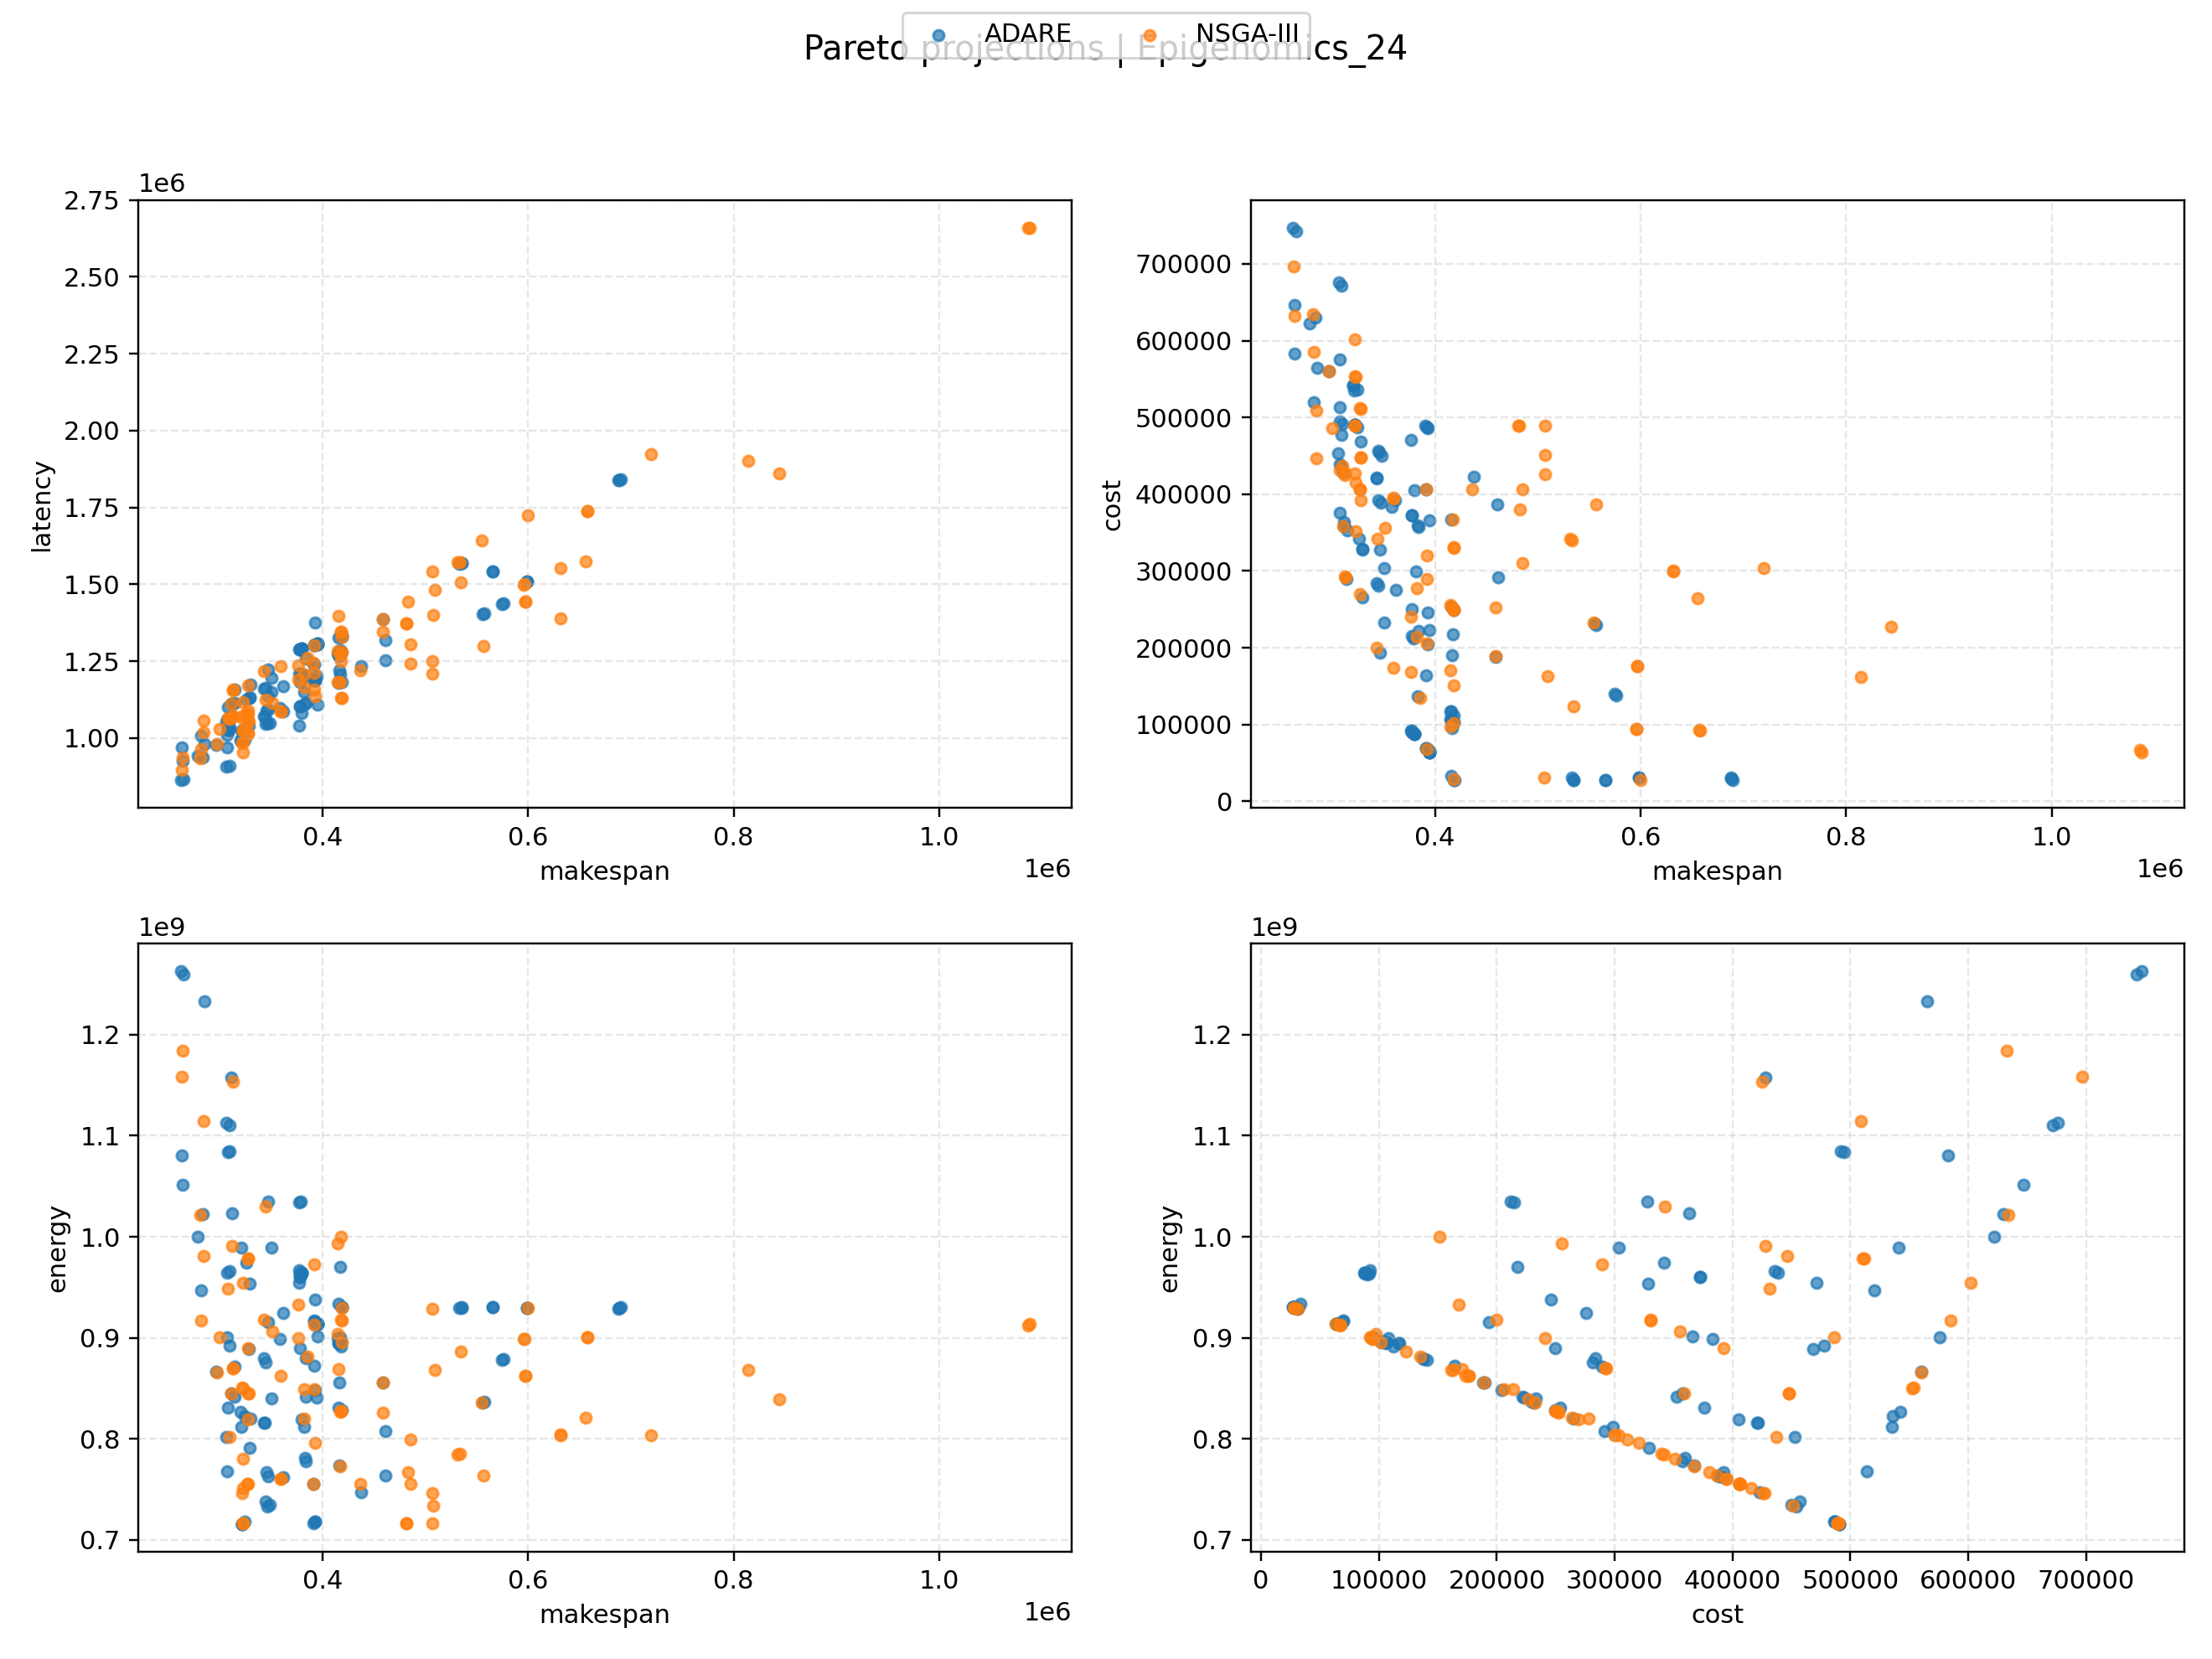
\includegraphics[width=0.32\textwidth]{Figures/pareto_test_epigenomics24.png}}
\caption{Pareto projections regenerated from the latest 6-run test campaign.}
\label{fig:pareto_latest}
\end{figure*}

\begin{figure*}[t]
\centering
\subfloat[Montage\_25]{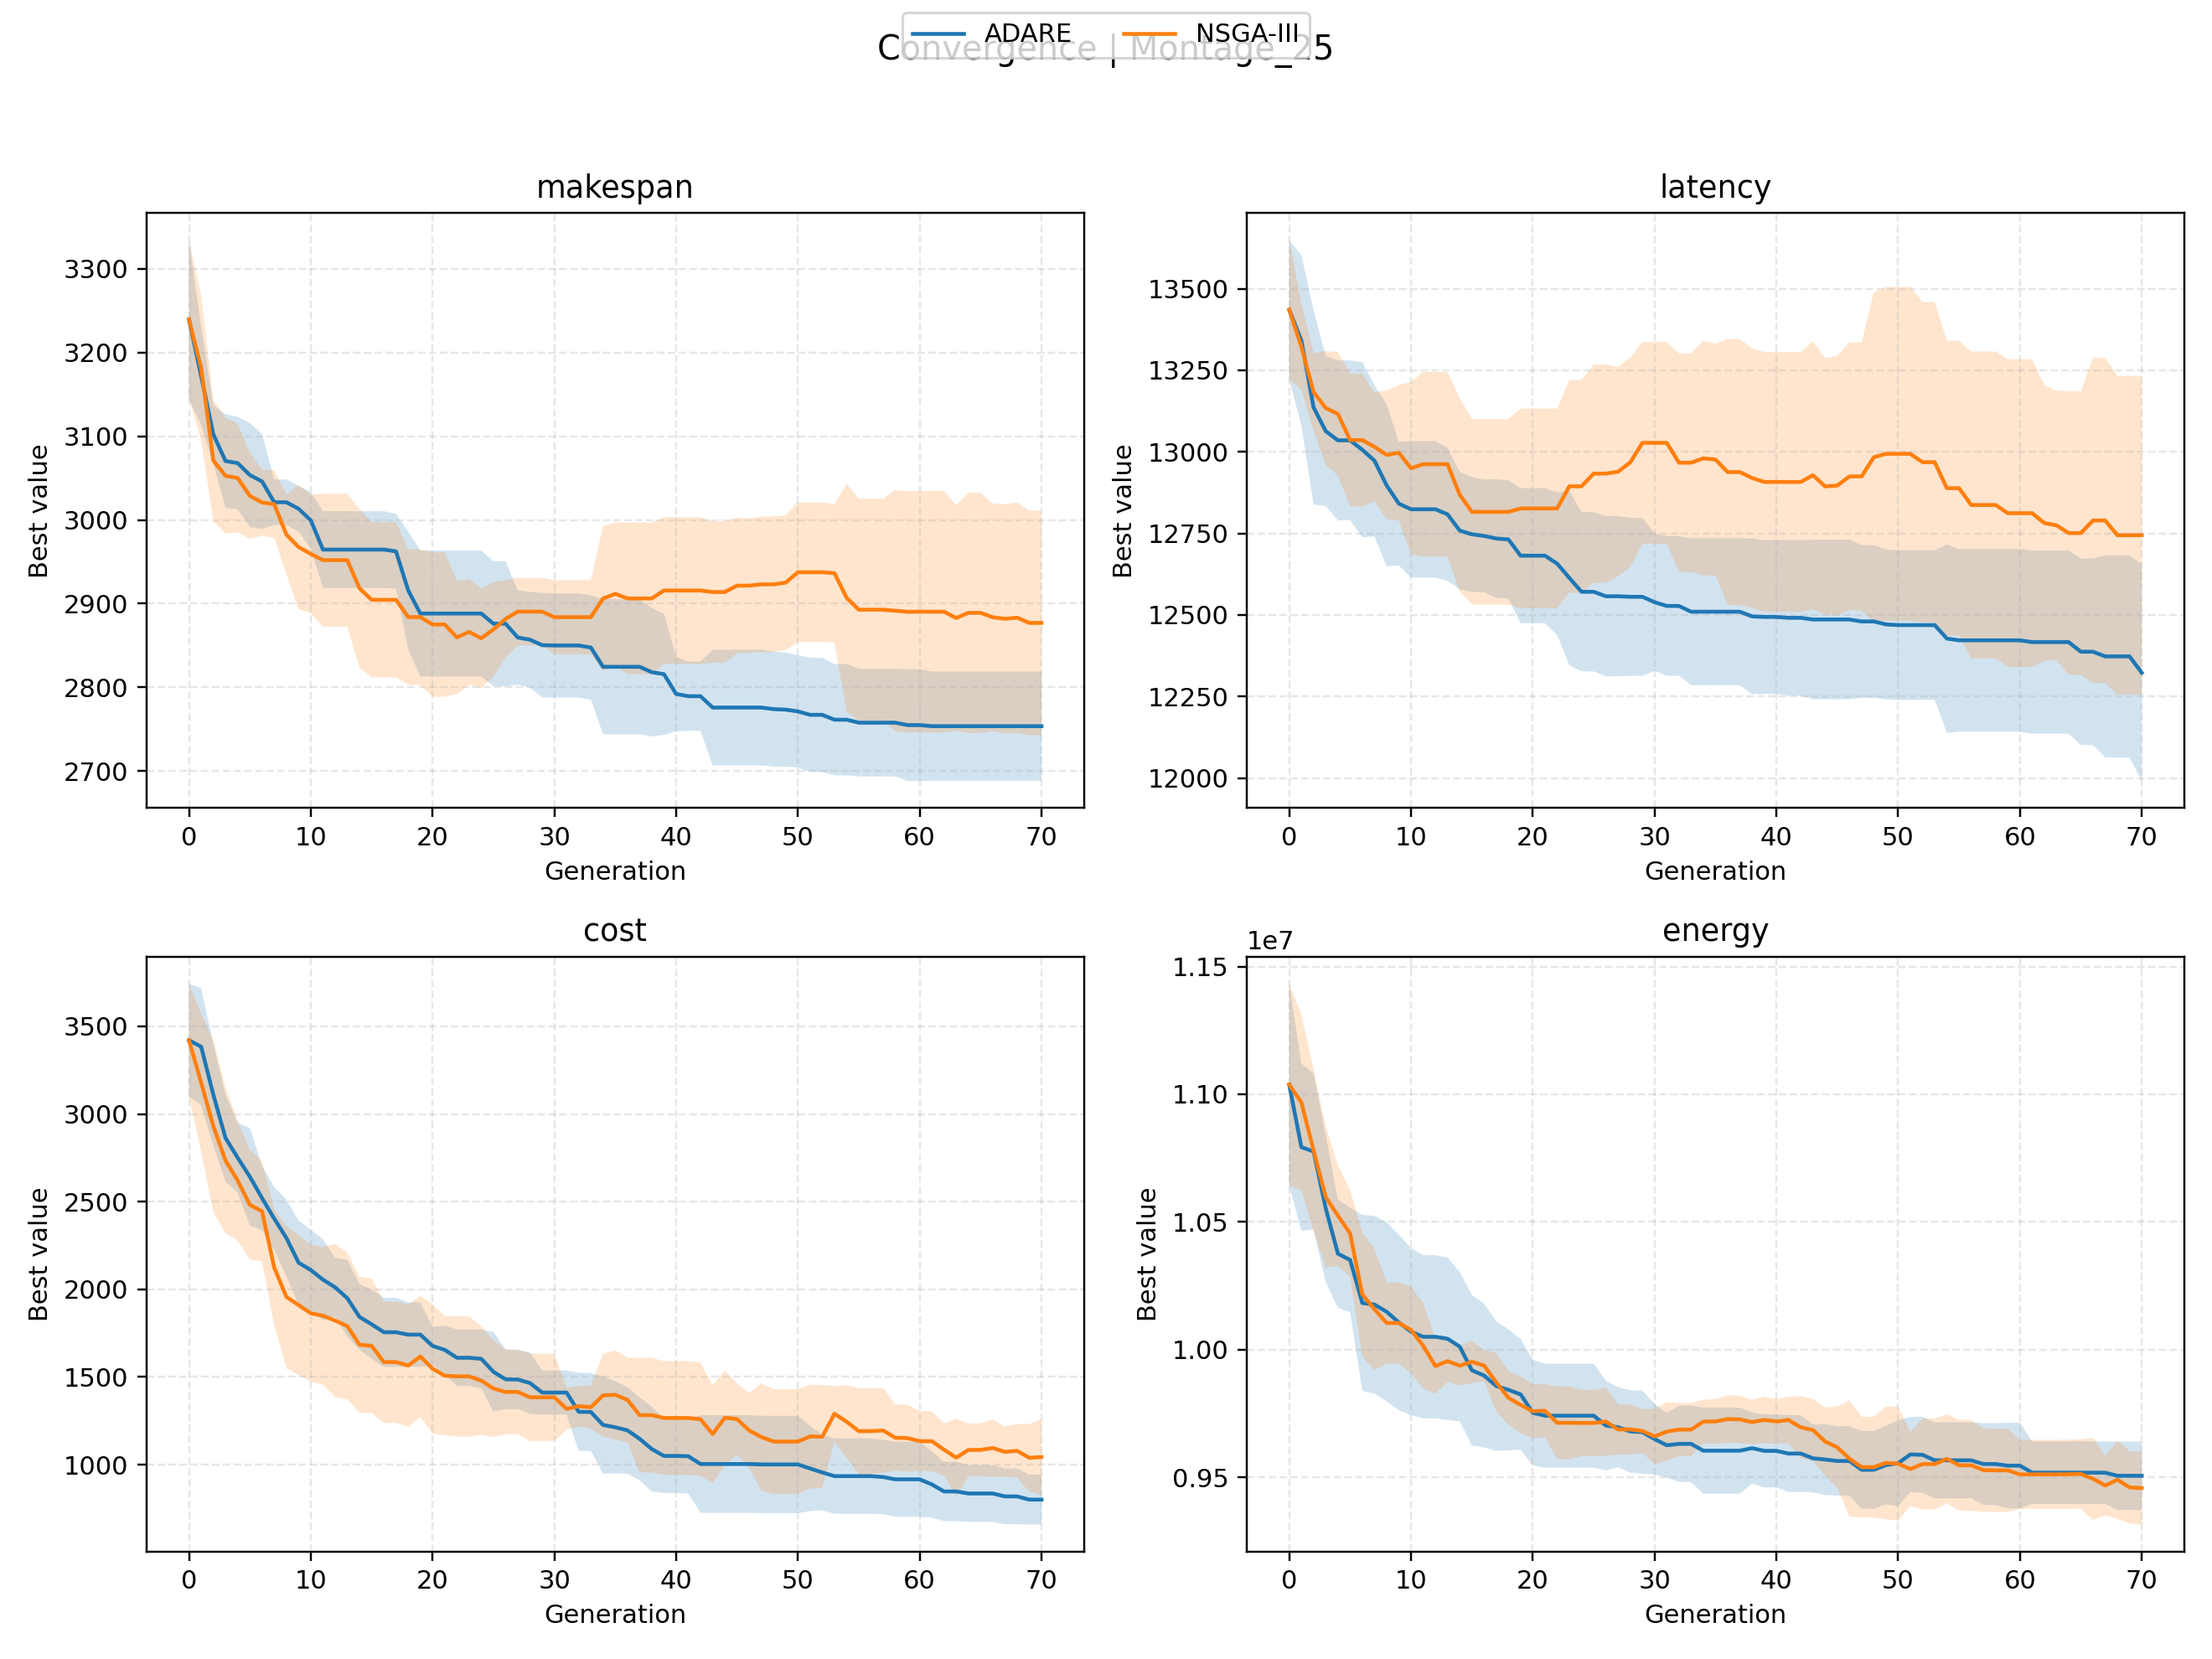
\includegraphics[width=0.32\textwidth]{Figures/convergence_test_montage25.png}}
\hfill
\subfloat[CyberShake\_30]{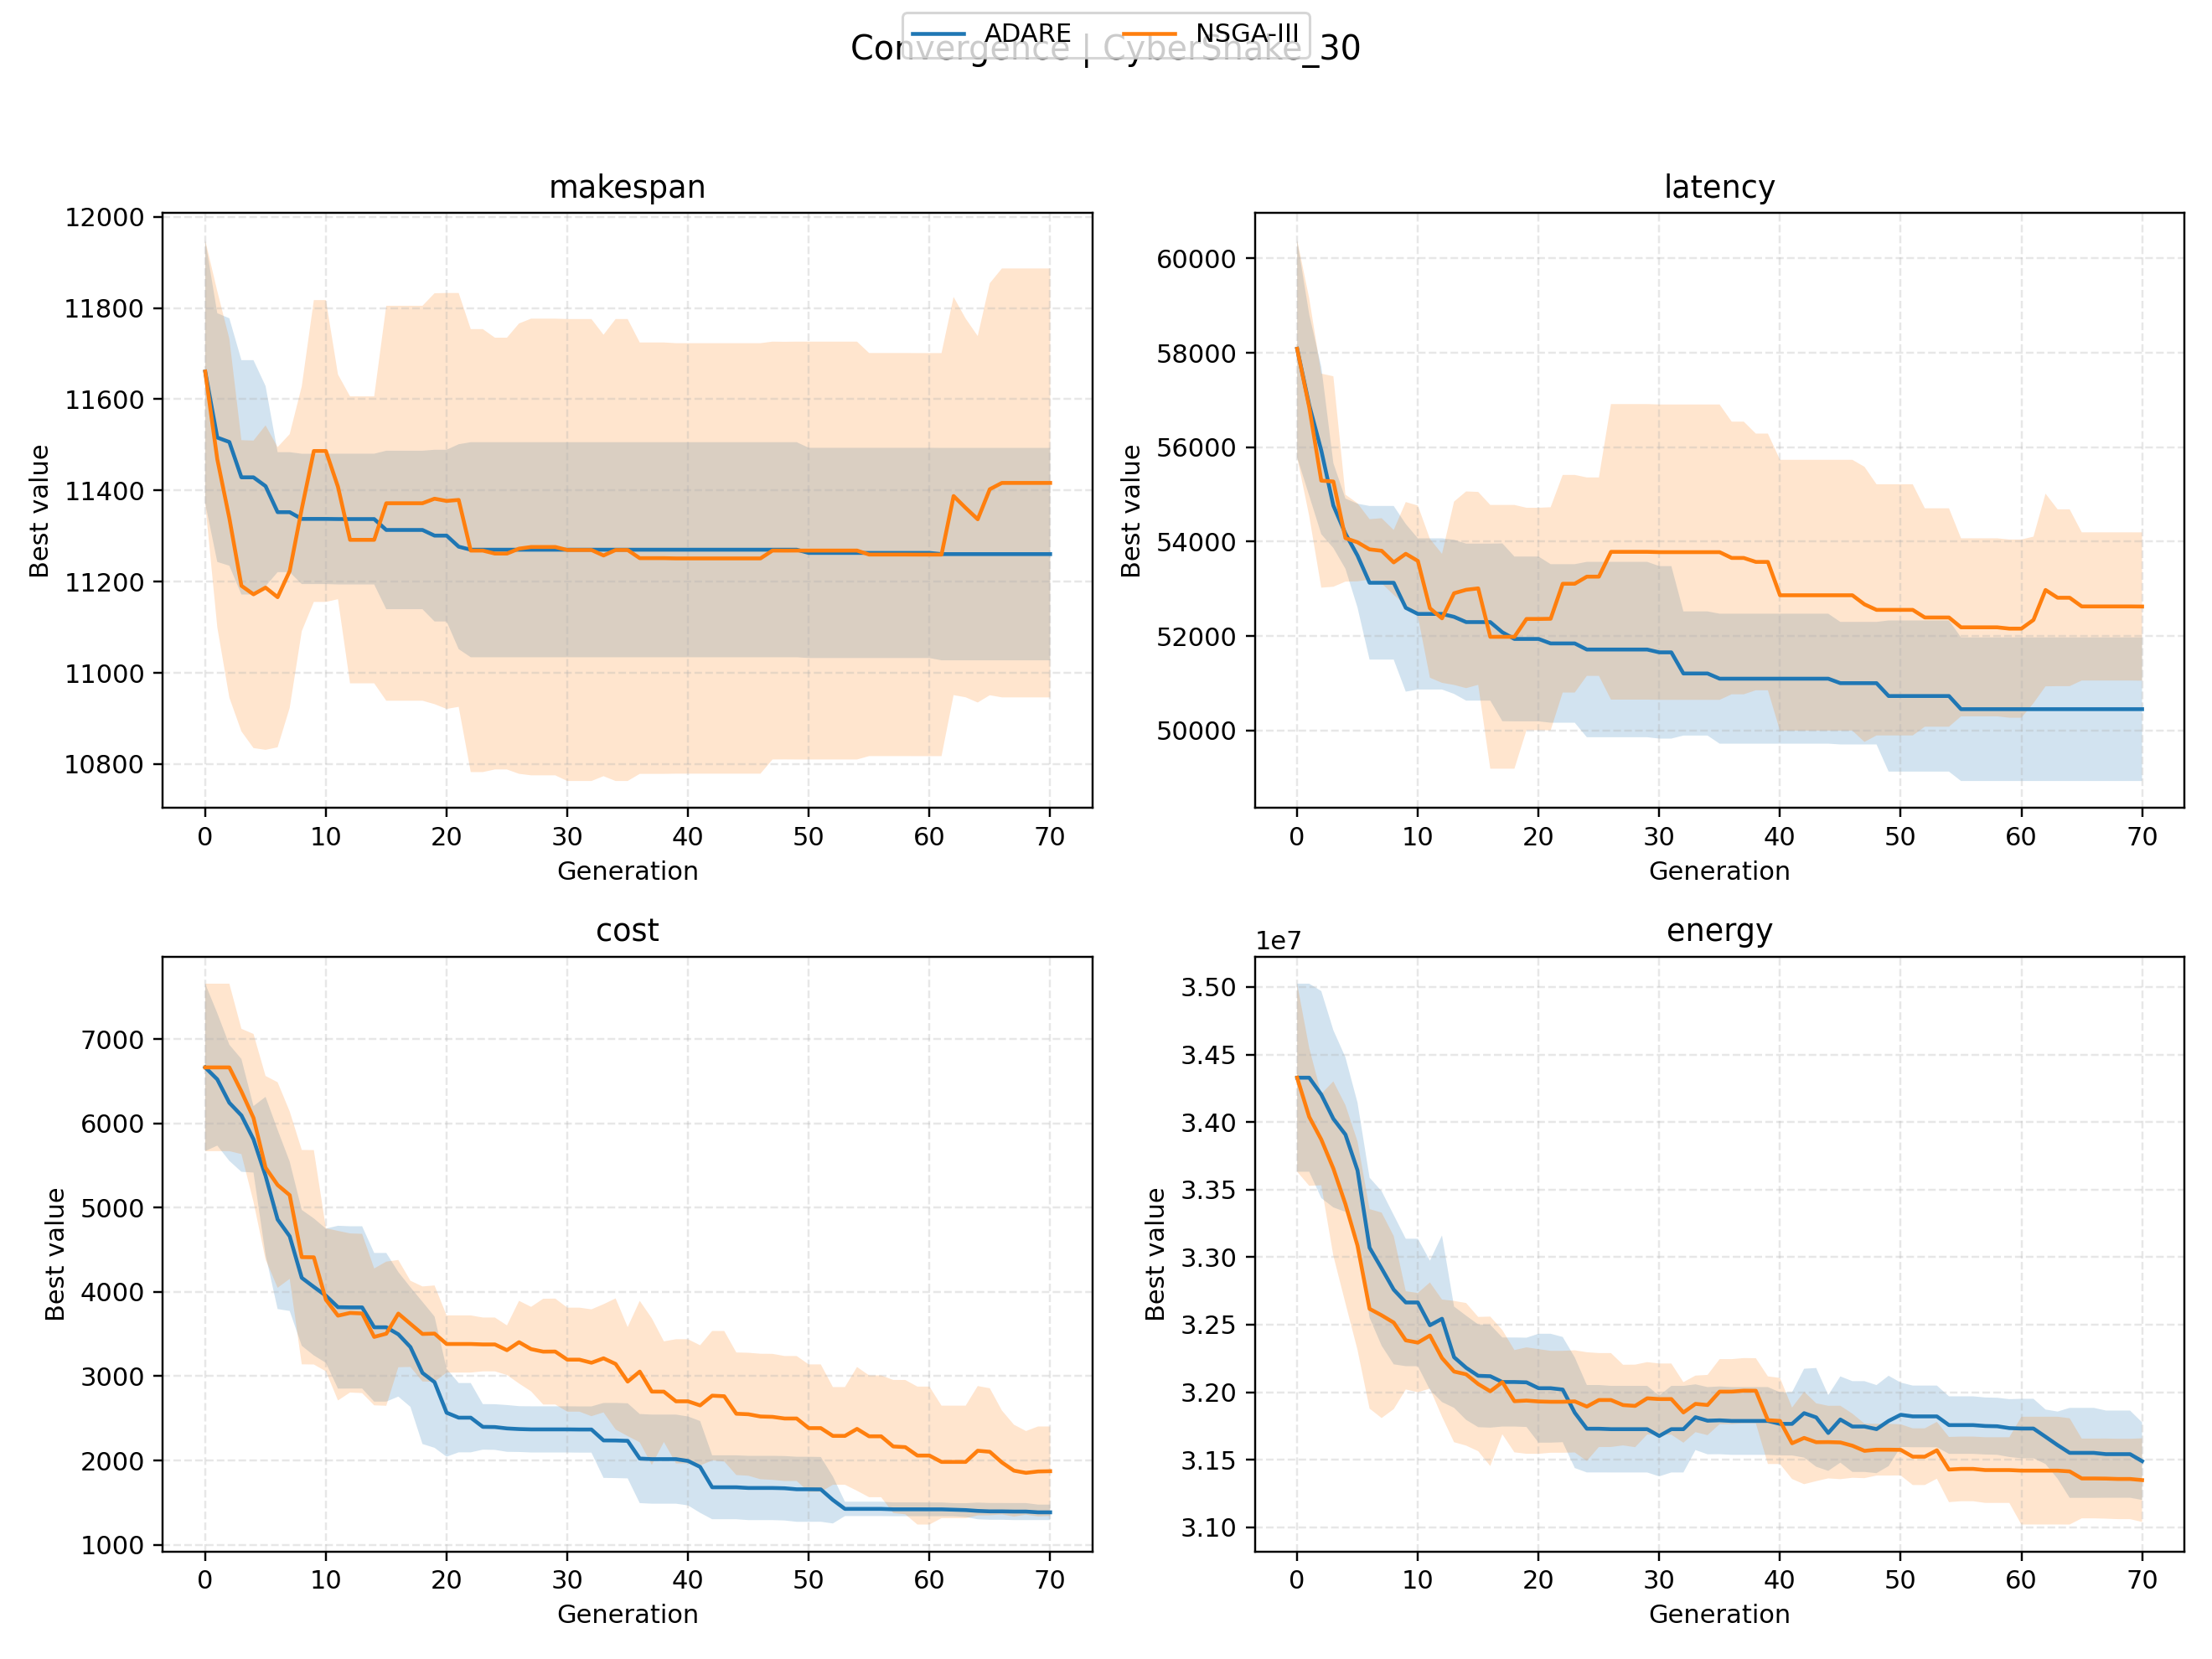
\includegraphics[width=0.32\textwidth]{Figures/convergence_test_cybershake30.png}}
\hfill
\subfloat[Epigenomics\_24]{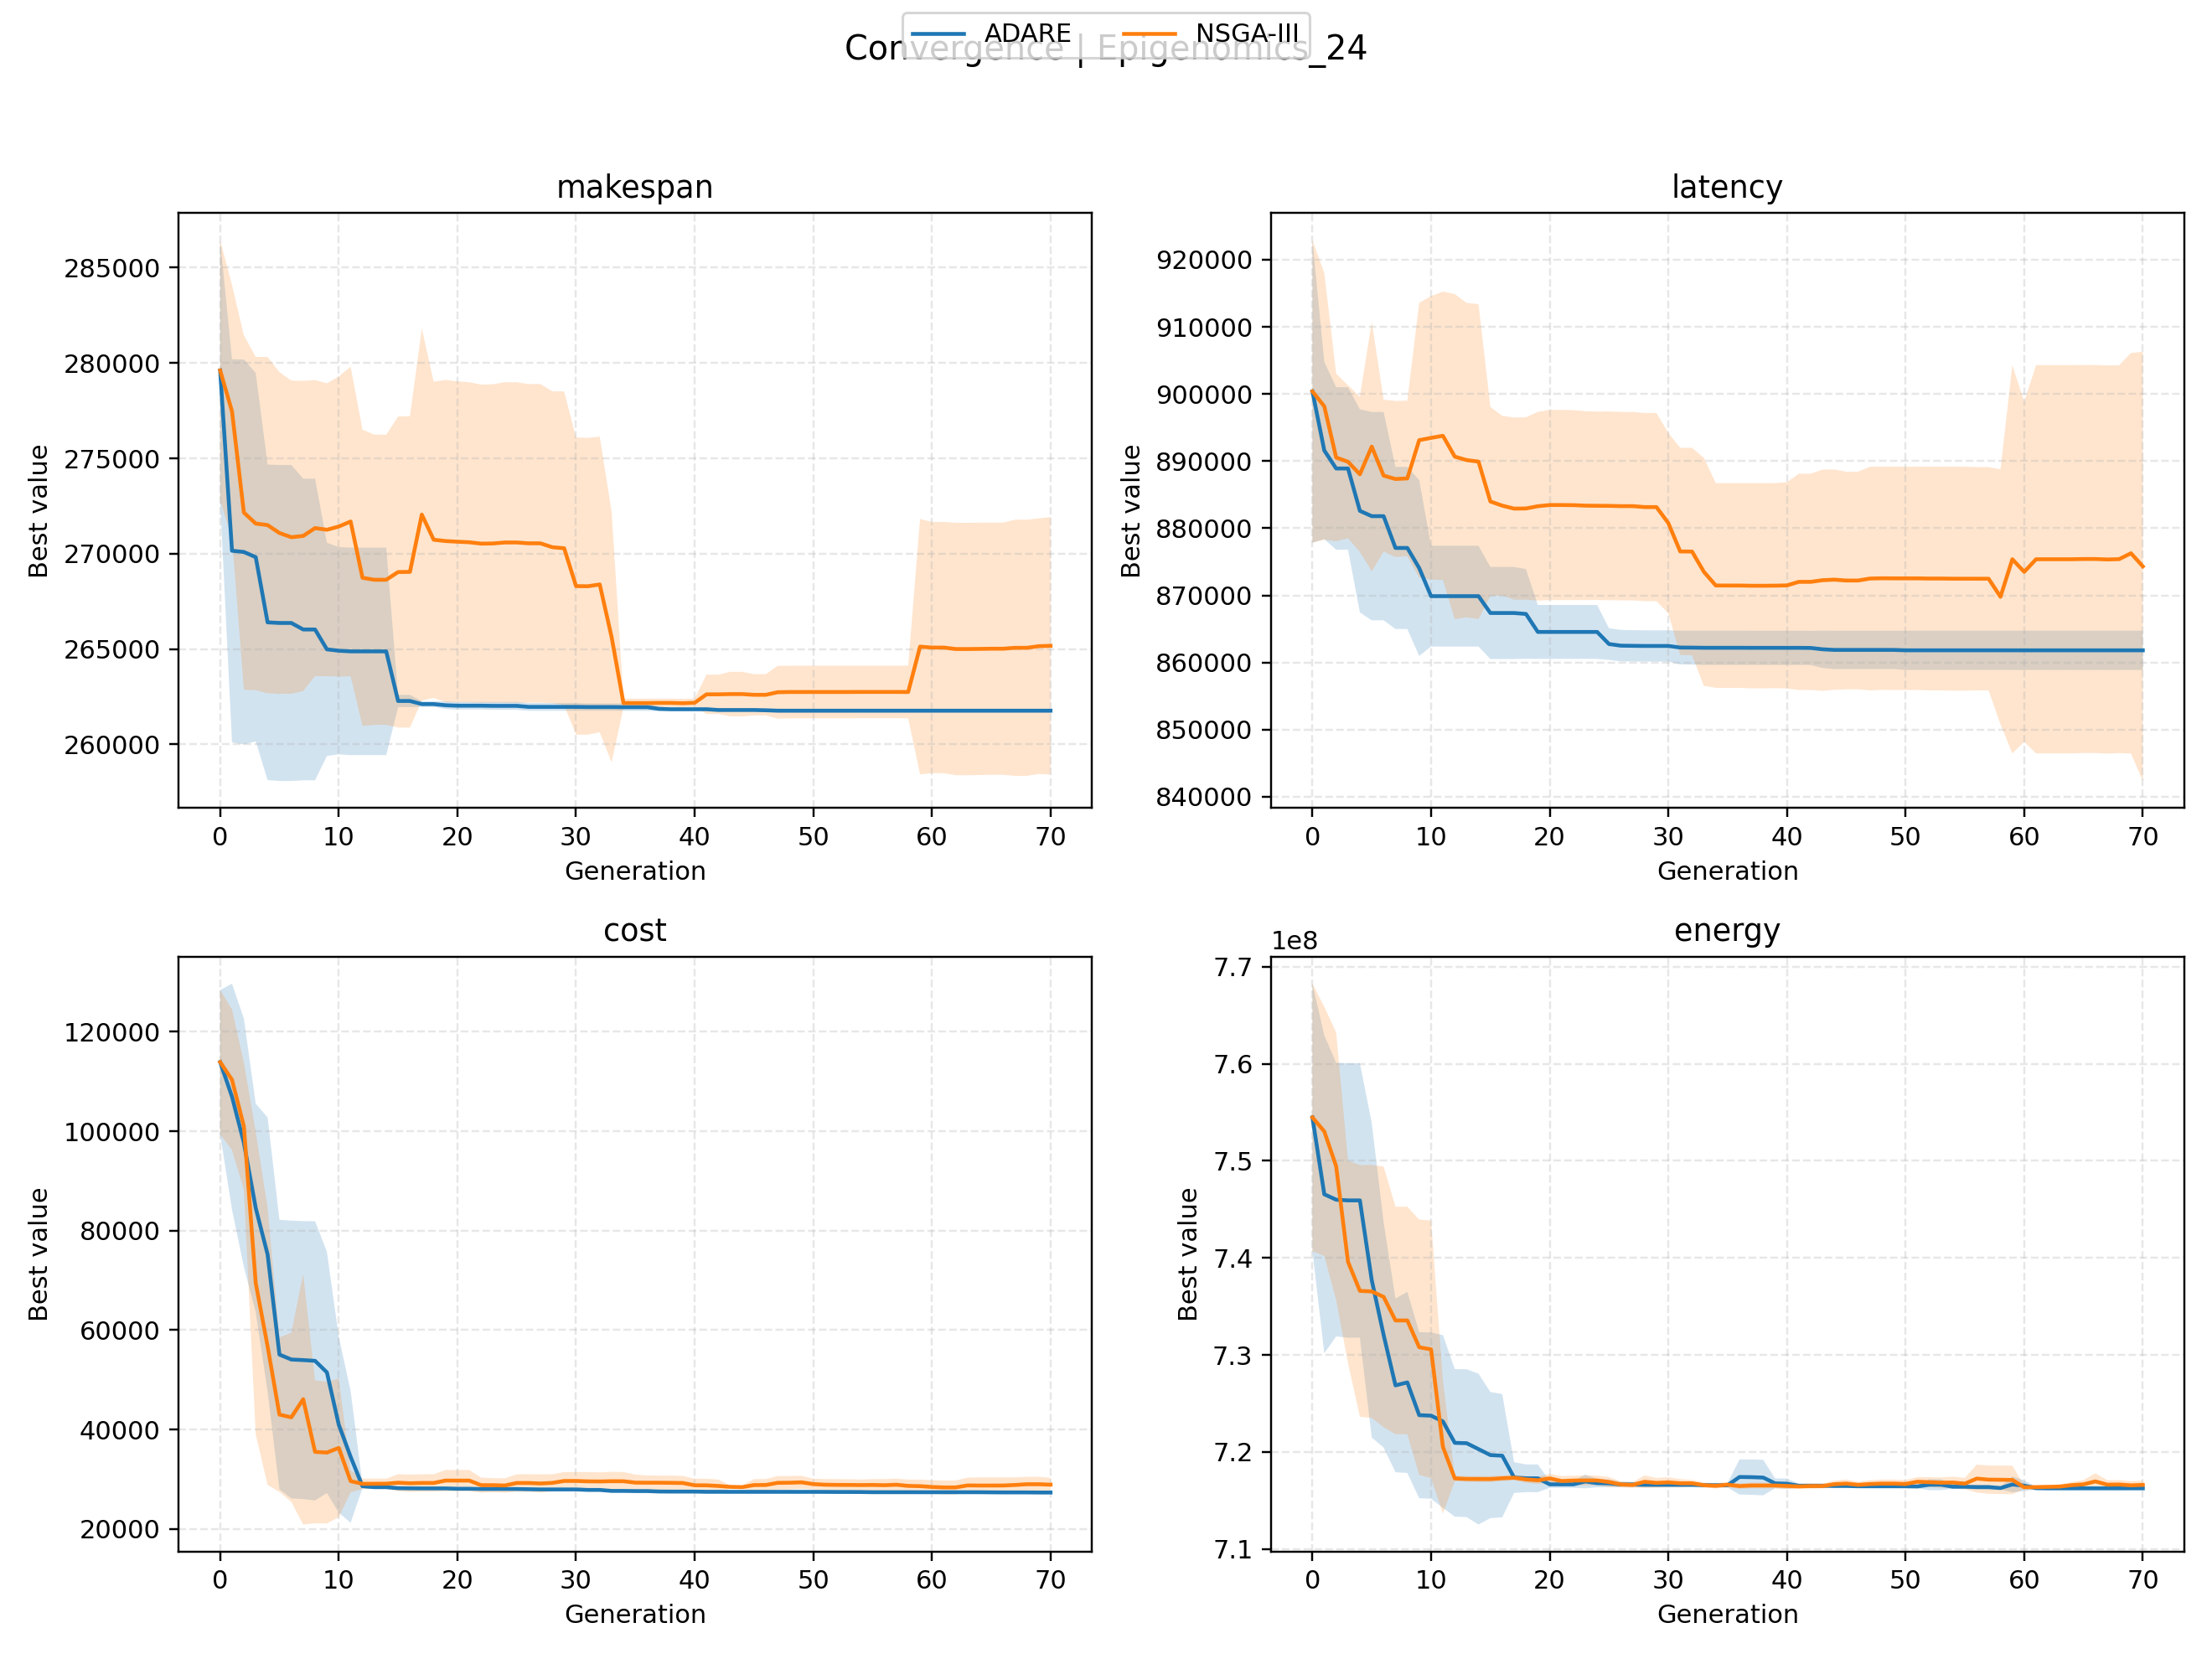
\includegraphics[width=0.32\textwidth]{Figures/convergence_test_epigenomics24.png}}
\caption{Convergence curves regenerated from the latest 6-run test campaign.}
\label{fig:convergence_latest}
\end{figure*}

Pareto and convergence plots agree : ADARE covers more interesting and exploitable trade-off zones and reaches higher extreme values. All of this while maintaining its speed across all three benchmarks.

\subsection{Metric-by-Metric Interpretation}
The global improvements are not caused by a single indicator.
HV, IGD, spacing and epsilon all progress across the three workflows. This is an excellent demonstration of better convergence and a good maintenance of diversity.
Coverage gains are exceptionally significant when it comes to Epigenomics\_24 and Montage\_25. ADARE outperforms a larger portion of the solutions generated by NSGA-III in these cases.

Runtime remains positive across the three workflows, despite the adaptive controls and the archive logic.
This is mainly explained by the dynamic operator selection and a controlled mutation budget, which avoid costly and unnecessary transformations in the late generations.

The most significant gains on extreme objective values appear on cost and latency in CyberShake\_30. Regarding Montage\_25, we have a strong improvement of the Makespan.
Gains are more modest for Epigenomics\_24 on energy\_best, but they remain positive and stable regardless of the run.

\subsection{Significance Overview}
\begin{table}[htbp]
\centering
\caption{Significant Wins Summary (Wilcoxon, $p<0.05$)}
\label{tab:significance}
\begin{tabular}{lcc}
\toprule
\textbf{Benchmark} & \textbf{All Quality} & \textbf{Core Quality} \\
\midrule
Montage\_25 & 4/6 & 3/5 \\
CyberShake\_30 & 3/6 & 2/5 \\
Epigenomics\_24 & 4/6 & 3/5 \\
\midrule
\textbf{Total} & \textbf{11/18} & \textbf{8/15} \\
\bottomrule
\end{tabular}
\end{table}

These 6 paired runs already allow us to observe significant differences on several metrics, but not on all of them.
This is a normal behavior in multi-objective scheduling : some metrics (such as spacing or epsilon) can vary more from one run to another depending on the shape of the Pareto front.
Increasing the number of runs and testing other workflow sizes would certainly help stabilize the statistical conclusions even further.

\subsection{Practical Takeaways}
From an engineering standpoint, ADARE can easily replace NSGA-III. This could be particularly interesting in cases where the scheduler must produce both a good front and reliable extreme candidates.
The final candidate per objective mechanism is particularly useful in production-close contexts, with operators being able to focus on a critical metric (a deadline or a response time) while keeping alternative trade-offs accessible.

\subsection{Reproducibility Notes}
Main command used for the test (instead of a "make" command):
\begin{itemize}
    \item \texttt{python main.py --benchmarks Montage\_25}\\
    \texttt{CyberShake\_30 Epigenomics\_24 --runs 6}
\end{itemize}
Generated reports:
\begin{itemize}
    \item \texttt{output/summary/}\\
          \texttt{global\_comparison\_report.txt}
    \item \texttt{output/<workflow>/reports/}\\
          \texttt{*\_comparison\_report.txt}
\end{itemize}
Generated figures used in this paper:
\begin{itemize}
    \item \texttt{Figures/pareto\_test\_montage25.png}
    \item \texttt{Figures/pareto\_test\_cybershake30.png}
    \item \texttt{Figures/pareto\_test\_epigenomics24.png}
    \item \texttt{Figures/convergence\_test\_montage25.png}
    \item \texttt{Figures/convergence\_test\_cybershake30.png}
    \item \texttt{Figures/convergence\_test\_epigenomics24.png}
\end{itemize}

\subsection{Threats to Validity}
Tests are conducted on three representative workflow families, but it would be worth testing more sizes and different infrastructure profiles.
Also, statistically significant data comes with a larger number of runs. 6 runs constitute a good base, but this is not a definitive ceiling for drawing solid conclusions.

\section{Conclusion}
The comparative study we conducted demonstrates that ADARE improves over NSGA-III through three concrete algorithmic contributions : an adaptive crossover control, a density-sensitive mutation, and an archive-guided final selection mechanism.
With a fair protocol, ADARE remains superior in quality and runtime across all three workflow families. We believe that an adaptive model is the answer to the extremely heterogeneous nature of environments.

\begin{thebibliography}{00}
\bibitem{deb2014}
K. Deb, \textit{Multi-Objective Optimization Using Evolutionary Algorithms}. Wiley, 2014.

\bibitem{deb2014nsga3}
K. Deb and H. Jain, ``An Evolutionary Many-Objective Optimization Algorithm Using Reference-Point-Based Nondominated Sorting Approach, Part I,'' \textit{IEEE Trans. Evol. Comput.}, vol. 18, no. 4, pp. 577--601, 2014.

\bibitem{durillo2014}
J. Durillo et al., ``Multi-objective workflow scheduling in cloud systems,'' \textit{Future Generation Computer Systems}, 2014.

\bibitem{xu2018}
X. Xu et al., ``Many-objective scheduling with NSGA-III variants,'' \textit{Applied Soft Computing}, 2018.

\bibitem{wu2019}
H. Wu et al., ``A Survey of Task Scheduling in Cloud and Fog Computing,'' \textit{Future Generation Computer Systems}, 2019.

\bibitem{goudarzi2021}
M. Goudarzi et al., ``Resource Management in Fog/Edge Computing: A Survey,'' \textit{ACM Computing Surveys}, 2021.
\end{thebibliography}

\end{document}
